\chapter{Robust adaptive phase-shifting demodulation for testing moving 
wavefronts}

%\section{Motivatio}
%Optical interferometer setups are very sensitive when environment
%perturbations affect its optical path. The wavefront under test is not
%static at all. In this paper, it is proposed a novel and robust phase-shifting
%demodulation method. This method locally estimates the interferogram’s
%phase-shifting, reducing detuning errors due to environment perturbations
%like vibrations and/or miscalibrations of the Phase-Shifting Interferometry
%setup. As we know, phase-shifting demodulation methods assume that the
%wavefront under test is static and there is a global phase-shifting for all
%pixels. The phase-shifting demodulation method presented here is based on
%local weighted least-squares, letting each pixel have its own phase-shifting.
%This is a different and better approach, considering that all previous works
%assume a global phase-shifting for all pixels of interferograms. Seeing this
%method like a black box, it receives an interferogram sequence of at least 3
%interferograms and returns the modulating phase or wavefront under test.
%Here it is not necessary to know the phase shifts between the interferograms.
%It does not assume a global phase-shifting for the interferograms, is robust
%to the movements of the wavefront under test and tolerates
%miscalibramiscalibrations of the optical setup with at least three
%interferograms in the sequence.

Optical interferometer setups are very sensitive when environment
perturbations affect its optical path. The wavefront under test is not
static at all. In this chapter, we propose a novel and robust phase-shifting
demodulation method. This method locally estimates the interferogram's
phase-shifting, reducing detuning errors due to environment perturbations
like vibrations and/or mis-calibrations of the PSI setup. 
As we know, phase-shifting demodulation methods assume that the
wavefront under test is static and there is a global phase-shifting for all
pixels. The phase-shifting demodulation method presented here is based on
local weighted least-squares, letting each pixel have its own phase-shifting.
This is a different and better approach, considering that all previous works
assume a global phase-shifting for all pixels of interferograms. Seeing this
method like a black box, it receives an interferogram sequence of at least 3
interferograms and returns the modulating phase or wavefront under test.
Here, as the method explained before, it is not necessary to know the phase 
shifts between the interferograms.
It does not assume a global phase-shifting for the interferograms, is robust
to the movements of the wavefront under test and tolerates
mis-calibrations of the optical setup with at least three
interferograms in the sequence.

\section{Introduction}
PSI is a very known technique designed for
testing static wavefronts. In PSI, it is generated an interferogram sequence of
at least 3 interferograms with a phase shifting between them. To recover the
modulating phase the well known phase-shifting demodulation methods are used
\cite{Bruning:74,Morgan,Schwider:83,Cheng:85,Hariharan:87,Estrada:09}. When the
wavefront under test remains static and the phase
shifts are introduced correctly, these phase-shifting methods recover the
modulating phase without error. However, in optical interferometer setups the
optical path is easily affected by environment perturbations. When environment
perturbations exist, the wavefront under test is moving and the phase-shifting
algorithms introduce an unavoidable detuning error
\cite{Servin:09,GeneralTheory}. Nowadays, we can deal
with a moving wavefront by taking all the interferograms in the same instant of
time, for example, by using pixelated polarized cameras \cite{Servin:10,
Kimbrough:06}. But, today this technology is expensive and is patent protected.
To deal with the mis-calibrations of the optical set up, previous works propose
self-tuning phase-shifting demodulation methods
\cite{Xu:06,Wang:04,Estrada:10}. However, all the previous
published works for PSI assume that the wavefront under test remains static and
there is a global phase-shifting for all pixels of the interferograms. This is
not true when environment perturbations affects the wavefront under test.
Suppose that you have a PSI optical setup, but, the wavefront under test is
perturbed by the environment in such a way that it is moving. The method
presented here is a robust adaptive phase-shifting demodulation method that let
us demodulate the interferogram sequence tolerating the movements of the
wavefront under test and mis-calibrations from the PSI setup. This method allows
each pixel have its own phase-shifting, reducing considerably detuning errors
and improving the estimation of the modulating phase. To show the performance of
the Robust Adaptive Phase-Shifting (RAPS) method presented here, we will present
tests and results from simulated and experimentally obtained data.

\section{Robust Adaptive Phase-Shifting (RAPS)}
The interferometric phase-shifting signal for a single pixel has the classic
model found in all papers about phase-shifting. In that case, it is assumed that
all pixels has the same phase-shifting, therefore the interferometric signal for
any pixel is the following:
\begin{equation}
  I_k(x,y) = a(x,y)+b(x,y)cos[\phi_0(x,y) + \omega_0 k],
\end{equation}
where $I_k(x,y)$ is the $k$-interferogram of $M\times N$ pixels, $a(x,y)$ is its
background illumination, $b(x,y)$ its contrast or modulation term,
$\phi_0(x,y)$ is the wavefront under test and $\omega_0$ is the phase-shifting
introduced by the PSI system for all pixels. When the wavefront under test is
perturbed by environment, it is moving and the movements affects the phase shift
on each pixel of the interferograms in the following way:
\begin{equation}
  I_k(x,y) = a(x,y)+b(x,y)cos[\phi_0(x,y) + \eta_k(x,y) + \omega_0 k],
\end{equation}
where $\eta_k(x,y)$ is the environment perturbation. To process this
information, we are going to take $\eta_k(x,y)$ and $\omega_0$ as $\beta_k(x,y)
= \eta_k(x,y) + \omega_0 k$ in such a way that the interferogram sequence
can be rewritten as
\begin{equation}
  I_k(x,y) = a(x,y)+b(x,y)cos[\phi_0(x,y) + \beta_k(x,y)],
\end{equation}
where $\beta_k(x,y)$ represents the induced non-static phase-shifting variation
of the $k$-interferogram. Now, we are going to estimate the wavefront
$\omega_0(x,y)$ and the spatial $\beta_k(x,y)$ variations of each interferogram
of the sequence.

The Eq. (4.4) shows the least-squares cost function to recover the wavefront
under test $\omega_0(x,y)$; assuming that we know its spatial variations
$\beta_k(x,y)$ for each interferogram.
\begin{equation}
  E[a(x,y),f(x,y)]=\sum_{k=0}^{K-1}[a(x,y) + Re\{f(x,y) e^{i\beta_k (x,y)} \} -
I_k (x,y)]^2.
\end{equation}
In this equation, $i = \sqrt{-1}$ and $f(x,y)$ is a complex value for the
$(x,y)$ site. The operator $Re{\cdot}$ takes the real part of its argument,
that is, $Re\{z\} = \frac{1}{2} (z+z^*)$; being $z$ a complex value and $z^*$
its complex conjugate. $K$ is the number of interferograms. By minimizing (4.4)
with respect to $a(x,y)$ and $f(x,y)$, the wavefront under test (the modulating
phase) is recovered as before 
\begin{equation}
 \hat{\phi}(x,y)=angle[\hat{f}(x,y)],
\end{equation}
being $\hat{f}(x,y)$ the complex value that minimizes Eq. (4.4) at $(x,y)$ site.
To minimize Eq. (4.4) we solve the following linear system for each $(x,y)$
pixel:
\begin{multline}
\left(\begin{array}{ccc}
K & \sum c_{k}(x,y) & \sum s_{k}(x,y)\\
\sum c_{k}(x,y) & \sum c_{k}(x,y)^{2} & \sum c_{k}(x,y)s_{k}(x,y)\\
\sum s_{k}(x,y) & \sum c_{k}(x,y)s_{k}(x,y) & \sum s_{k}(x,y)^{2}
\end{array}\right)\left(\begin{array}{c}
\hat{a}(x,y)\\
\hat{\phi}(x,y)\\
\hat{\psi}(x,y)
\end{array}\right) = \\ \left(\begin{array}{c}
\sum I_{k}(x,y)\\
\sum I_{k}(x,y)C_{k}(x,y)\\
\sum I_{k}(x,y)S_{k}(x,y)
\end{array}\right).
\end{multline}
The sums run from $k = 0$ to $K=-1$, being $K$ the number of interferograms.
$\hat{\phi}(x,y)$ and $\hat{\psi}(x,y)$ are the real and imaginary parts of 
$\hat{f}(x,y)$, respectively. $c_k(x,y)$ and $s_k(x,y)$ are the real and
imaginary parts of $e^{i\beta_k(x,y)}$, respectively.

Now, in the Eq. (4.7) we propose the local weighted least-squares cost function
for estimating the wavefront variations $\beta_k(x;y)$ for the $(x,y)$ site at
the $k$-interferogram; assuming that the wavefront under test $\phi_0(x,y)$ is
known.
%%\begin{equation}
\begin{multline}
E[a(x,y),g_{k}(x,y)]= \\ \sum_{m=0}^{M-1}\sum_{n=0}^{N-1}\Bigg[\{a(m,n)+Re\{g_{k}(m,
n)e^ { i\phi_{0}(x,y)}\}-I_{k}(m,n)\}h(x-m,y-n)\Bigg]^{2}
\end{multline}
%%\end{equation}
In this equation, $h(x,y)$ is an scalar field that weights the least-squares
error of Eq. (4.7). By minimizing Eq. (4.7) with respect to $a(x,y)$ and
$g_k(x,y)$, the spatial wavefront variations $\beta_k(x,y)$ are recovered as
\begin{equation}
 \hat{\beta_k}(x,y)=angle[\hat{g_k(x,y)}],
\end{equation}
being $\hat{g_k(x,y)}$ the complex value that minimizes Eq. (4.7). The Eq. (4.7)
can be seeing like the convolution of the least-squares error with the kernel
$h(x,y)$. The kernel $h(x,y)$ weights the local neighborhood around the site
$(x,y)$ being processed. In this way, we have a weighted least-squares cost
function for each pixel $(x,y)$ and we can estimate the phase-shifting variation
$\beta_k(x,y)$ for each pixel $(x,y)$ of the $k$-interferogram. The linear
equation system that minimize Eq. (4.7), can be given in the following way:
\begin{multline}
 \left(\begin{array}{ccc}
[1s*h](x,y) & [\phi*h](x,y) & [\psi*h](x,y)\\{}
[\phi*h](x,y) & [\phi*h]^{2}(x,y) & [\phi\psi*h](x,y)\\{}
[\psi*h](x,y) & [\phi\psi*h](x,y) & [\psi*h]^{2}(x,y)
\end{array}\right)\left(\begin{array}{c}
\hat{a}(x,y)\\
\hat{c}_{k}(x,y)\\
\hat{s}_{k}(x,y)
\end{array}\right)= \\ \left(\begin{array}{c}
[I_{k}*h](x,y)\\{}
[I_{k}\phi*h](x,y)\\{}
[I_{k}\psi*h](x,y)
\end{array}\right)
\end{multline}
where $*$ is the convolution operator and $[*](x;y)$ means the convolution
evaluated at $(x,y)$. The term $1s$ is an scalar field of ones with dimension
$M \times N$. In this case, $\hat{\phi}(x,y)$ and $\hat{\psi}(x,y)$ are
the real and imaginary parts of $e^{i \phi_0(x,y)}$, respectively, and
$c_k(x,y)$ and $s_k(x,y)$ are the real and imaginary parts of $\hat{g}(x,y)$,
respectively.

Having the linear systems that estimate the wavefront under test $\phi_0(x,y)$
and its variations $\beta_k(x,y)$ for all pixels of all interferograms (Eqs.
(4.6) and (4.9) respectively), we use them iteratively in the following way:

\begin{itemize}
 \item[1] Set your convolution kernel $h(x,y)$ that will weight the local
 neighborhood around the $(x,y)$ sites. For example, $h(x,y)$ can be a mean or
 Gaussian window.
 \item[2] Start the process by setting initial values for $\beta_k(x,y),
 \forall (x,y),$ $k = 0,1,2,\dots,K-1$ being $K$ the number of interferograms.
 \item[3] Solve the linear system of Eq. (4.6) $\forall(x,y)$ and obtain 
 $\hat{\phi_0} (x,y)$ using Eq. (4.5).
 \item[4] For $k = 0,1,2,\dots,K-1$, use the previous wavefront estimation
 $\hat{\phi}_0 (x,y)$ to solve the linear equation system of Eq. (4.9)
 $\forall(x,y)$ and obtain $\hat{\beta}_k(x,y)$ using Eq. (4.8).
 \item[5] With the previously estimated $\hat{\beta}_k(x,y)$ of each
 interferogram, repeat subsequently the steps 3 and 4 until reach a convergence
 error.
\end{itemize}
As said in the step 5, this iterative process do its job until a convergence
error is reached. This converge error can be given as the relative error
between the values in a previous iteration and the values in the current
iteration in the following way:
\begin{equation}
 \varepsilon=\sum_{x,y}\mid\hat{\phi}_{0}^{+}(x,y)-\hat{\phi}_{0}^{-}(x,y)
 \mid,
\end{equation}
where $\hat{\phi}_{0}^{+}(x,y)$ is the phase obtained in the current iteration
and $\hat{\phi}_{0}^{-}(x,y)$ is the phase obtained in the previous iteration.
At the end of this process, $\hat{\phi}_{0}(x,y)$ and $\hat{\beta}_k(x,y)$
will have the best estimations of the wavefront under test and its non-constant
variations, respectively. The initial values in step 2 are important. By
experimenting numerically with simulations, we found the following initial
values as good starting points: $\hat{\beta}_k(x,y) = \frac{\pi}{2}k, 
\forall(x,y)$. We could use other value different to zero as starting point of
the iterative process, however, starting at $\pi/2$ is a good starting point
since in practice phase-shifting interferometers are calibrated to introduce
a phase shift of $\pi/2$ radians. Certainly, starting at $\pi/2$ is not always
the best if we have a priori information about the phase shifts introduced. For
example, if we know that the phase-shifting interferometer introduce $\pi/4$
phase shift radians, then the best starting point is $\pi/4$ radians.

\begin{figure}[th!]
	\begin{center}
		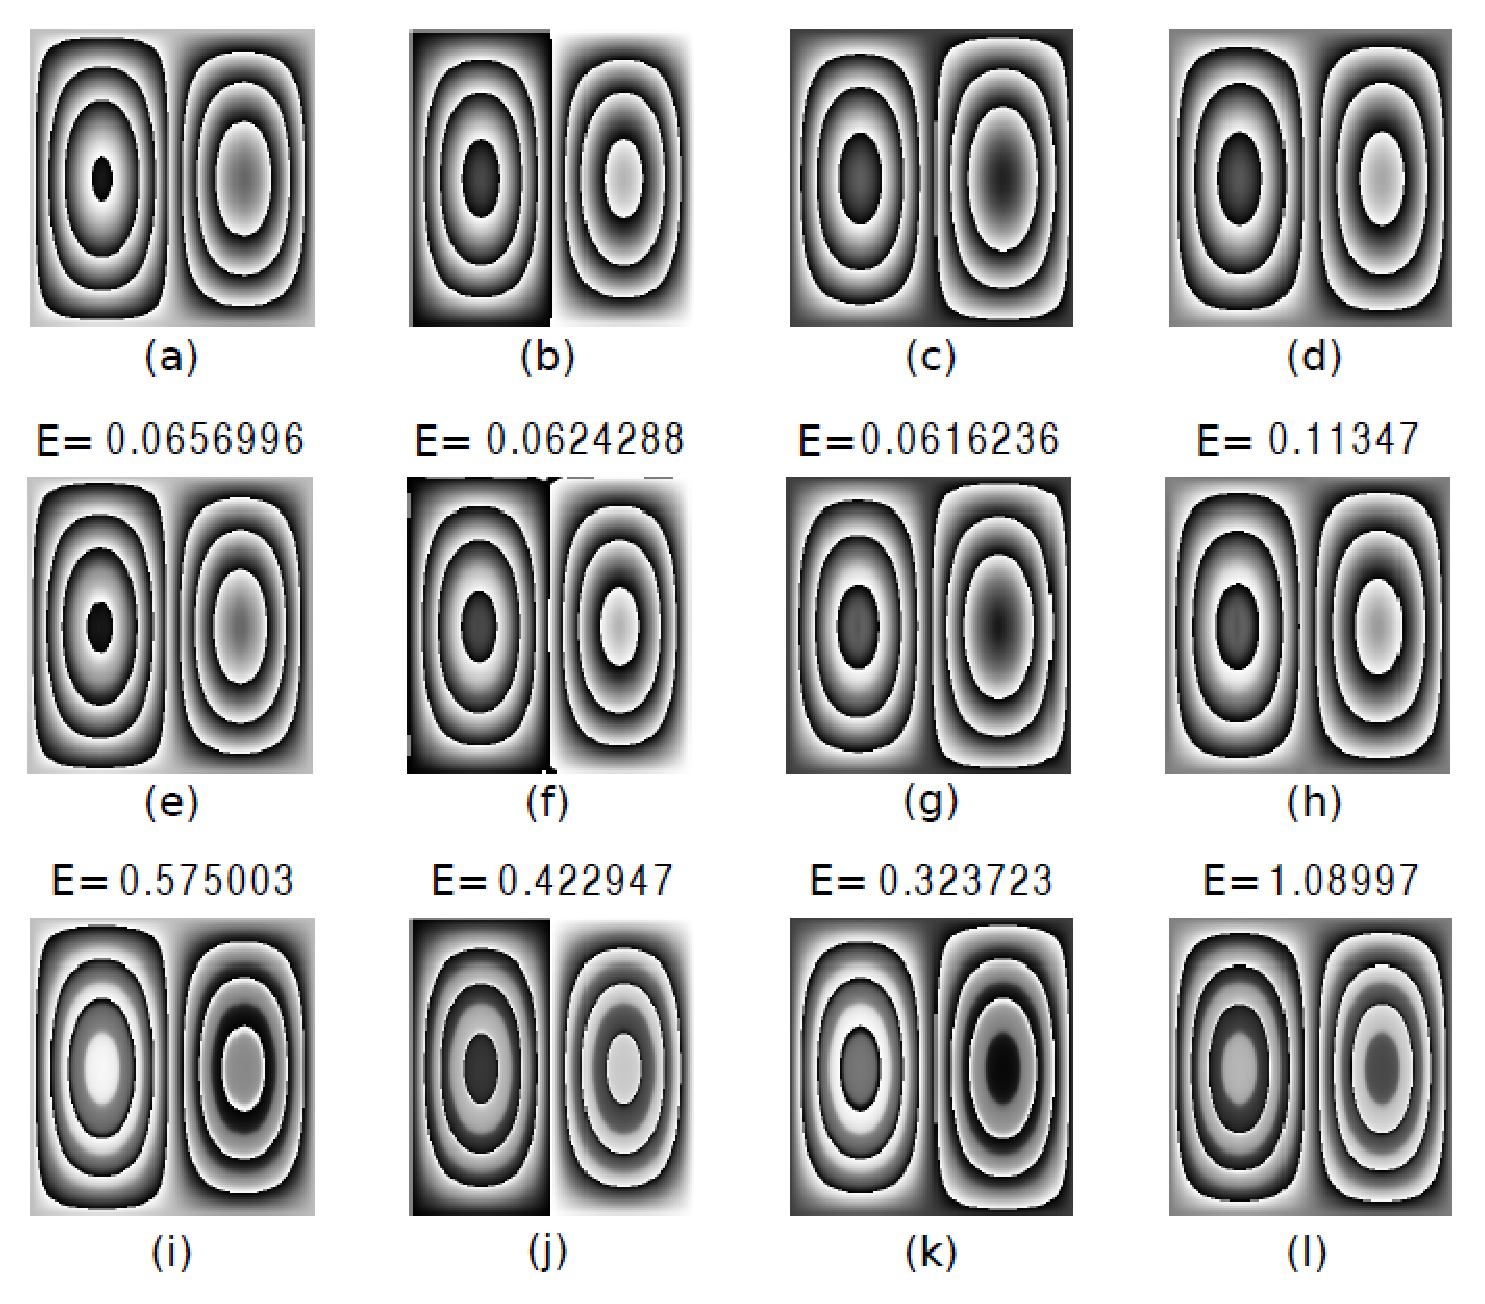
\includegraphics[scale=0.4]{Chpt3_figures/fig_1.eps}
	\end{center}
	\caption{Numerical examples.From (a) to (b) we show the wrapped
	wavefronts generated with Eq. (4.11). From (e) to (h) we show the
	estimated wavefronts using the RAPS algorithm presented here. From
	(i) to (l) we show the estimated wavefronts using the AIA. Above each
	estimated wavefront we show the estimation error.} 
	\label{fig:SimPhaseComparisonRAPS}
\end{figure}

\section{Tests and results}

In the following test, we are going to quantify the wavefront estimation error
of the RAPS demodulation method presented here. We are going to compare our
results with the estimation error that is obtained with the Advanced Iterative
Algorithm (AIA) presented in \cite{Wang:04}. For this test, we simulated a
moving wavefront and generated 4 interferograms with a phase-shifting of
$\pi/2$. The moving wavefront was modeled using a two-modes vibrating plate in
the following way:
\begin{equation}
 \phi_k (x,y) = A \cos \Big( \frac{2\pi}{256}x \Big) \sin \Big(
\frac{2\pi}{256}y \Big) \cos \Big( \frac{\pi}{17}k \Big)
\end{equation}
The Figs. 4.1(a-d) shows the wrapped wavefronts of this simulated moving
wavefront. Using the RAPS and the AIA method, we estimate the wavefront for each
interferogram and the results are shown at Figs. 4.1(e-h) and 4.1(i-l)
respectively. The global error of the phase estimation is shown above its
wrapped phase image and it was calculated in the following way
\begin{equation}
 \varepsilon = \sqrt{\frac{1}{M \times N} 
 \sum_{x=0}^{M-1} \sum_{x=0}^{M-1} 
 \mid \phi_{k}(x,y)-\hat{\phi}_{k}(x,y) \mid^2},
\end{equation}
where $\phi_{k}(x,y)$ and $\hat{\phi}_{k}(x,y)$ are the simulated and
estimated wavefronts for the $k$-interferogram, respectively, and the dimension
of interferograms is $M\times N = 256 \times 256$. For the RAPS method, the
kernel $h$ was a mean window of $32 \times 32$. By the estimated errors obtained
in each phase estimation (shown above each image of the estimated phase maps of
Fig. 4.1), we can see that the RAPS method reduces one order of magnitude the
estimation error, compared with an standard iterative phase-shifting algorithm
like the AIA. The computational time was 0.374 seconds for the AIA and 4.99
seconds for the RAPS method.

\begin{figure}[th!]
	\begin{center}
		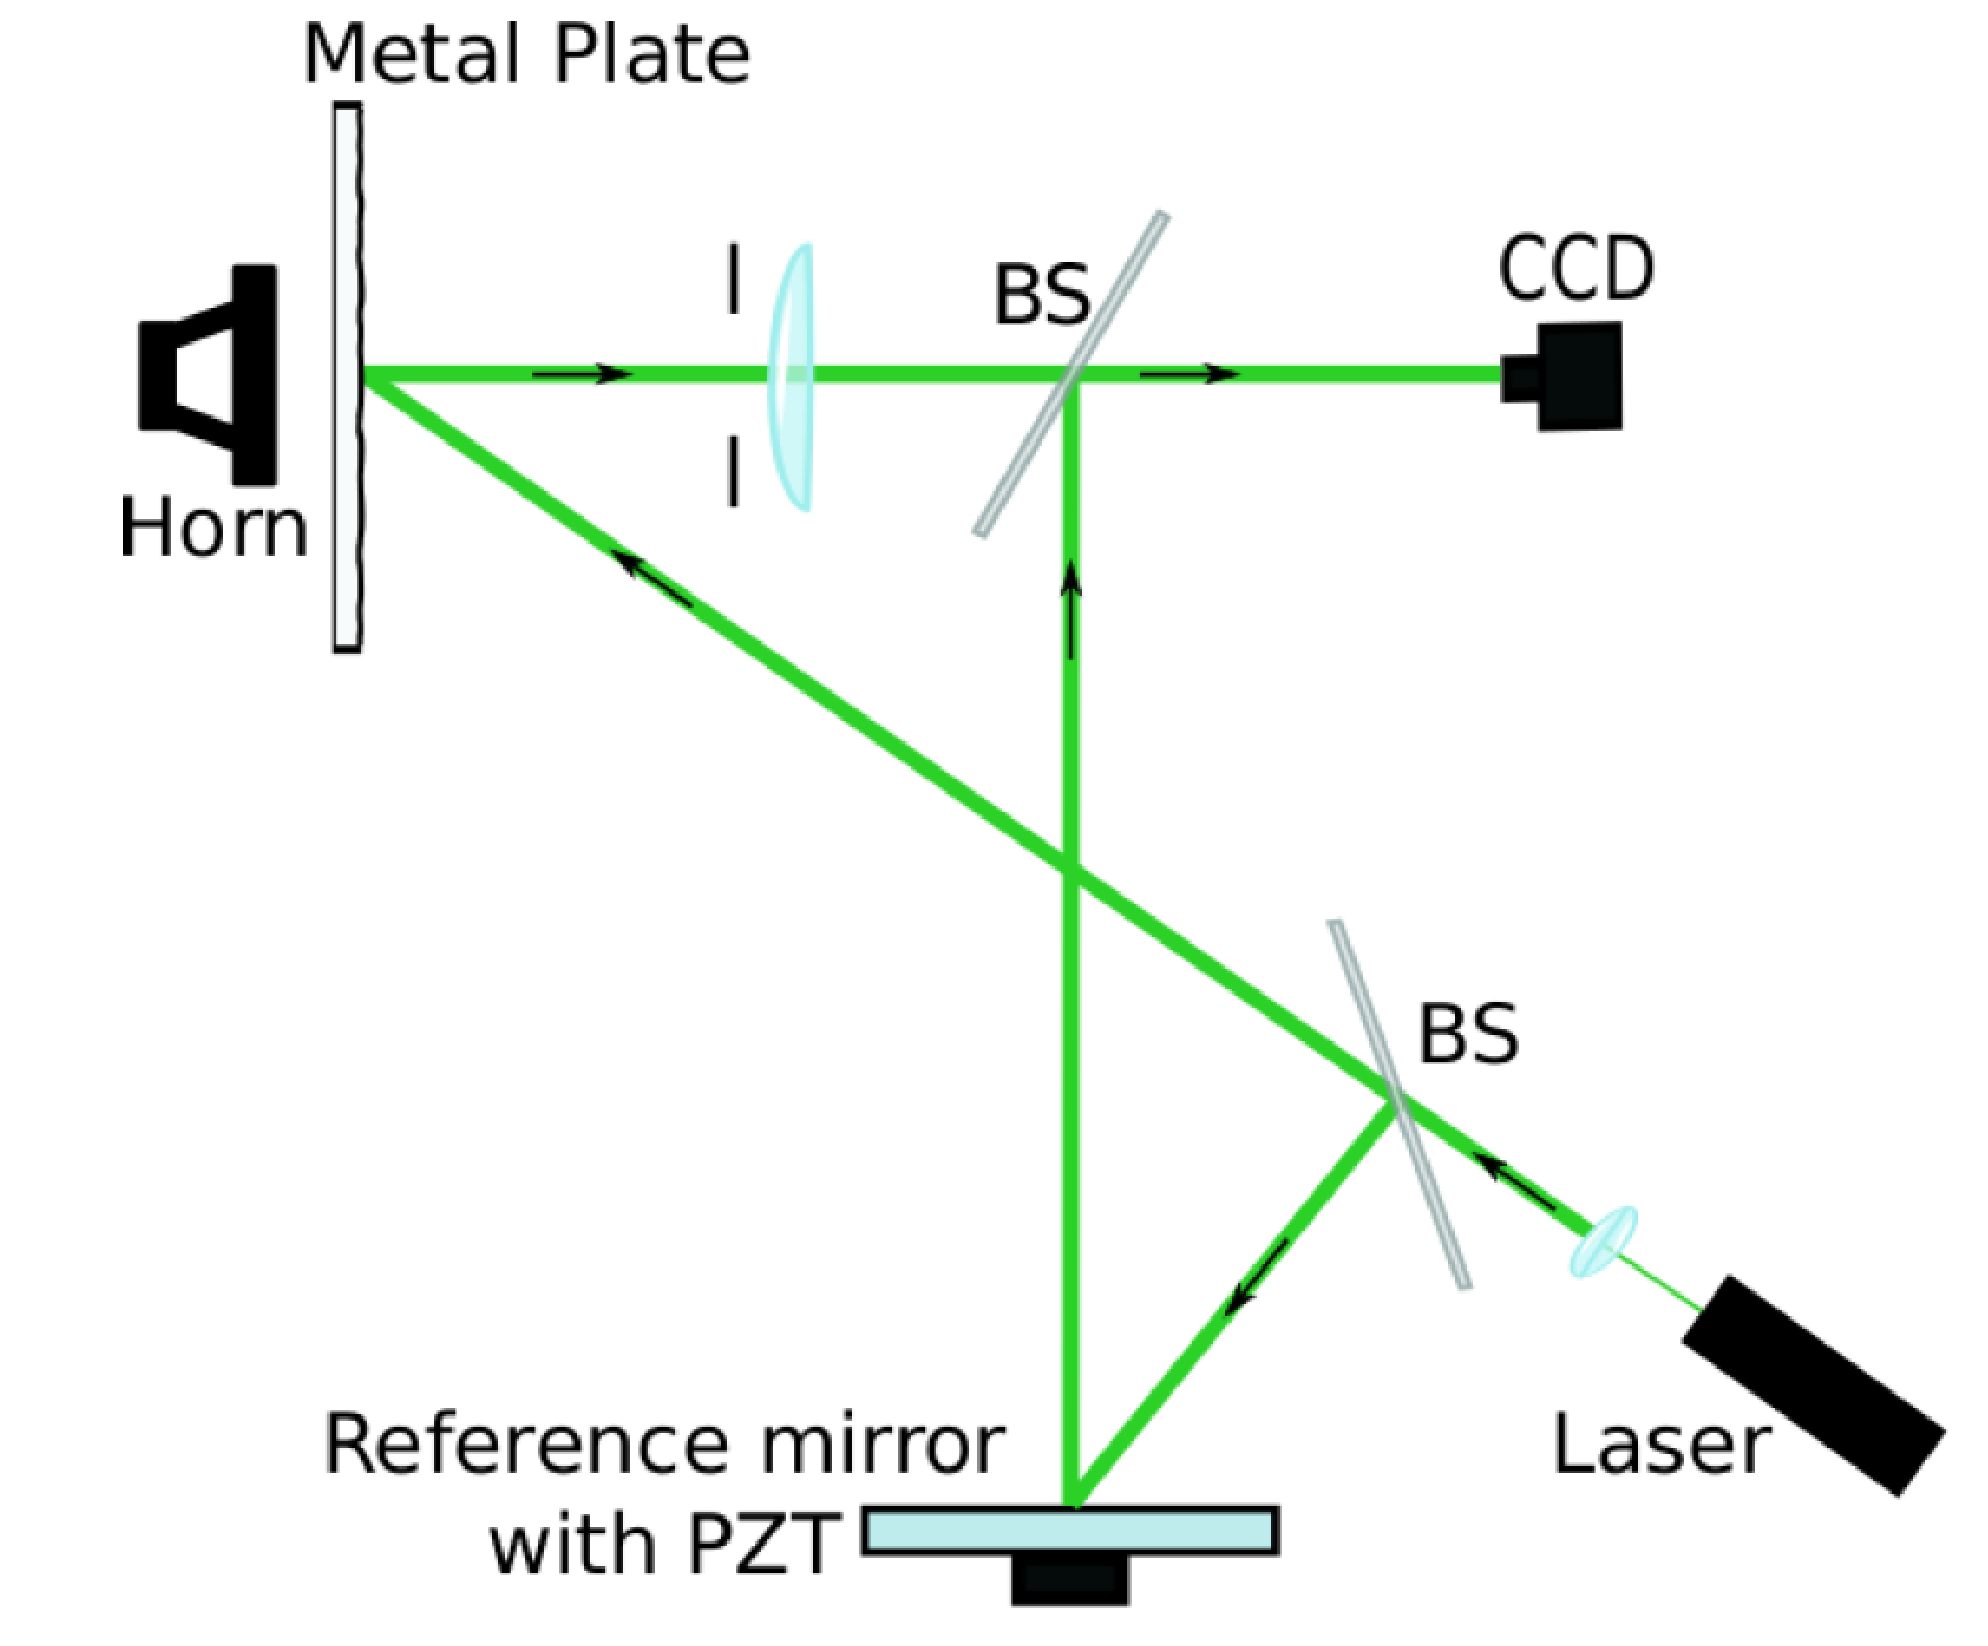
\includegraphics[scale=0.2]{Chpt3_figures/fig_2.eps}
	\end{center}
	\caption{Experimental setup.Electronic Speckle Pattern Interferometry
	(ESPI) setup. The object under test is a metal plate perturbed with a
	horn. The reference mirror has attached a piezoelectric transducer
	(PZT) as phase shifter.} 
	\label{fig:ExperimentalSetupRAPS}
\end{figure}

Now, we are going to test our method with interferograms experimentally obtained
and compare qualitatively the results with the AIA method. For this test, the
interferograms has a dimension of $480 \times 640$ and the kernel that we used
for the RAPS method was a mean window of $132\times 132$. The interferogram
sequence was generated by using the ESPI array like the shown in Fig. 4.2. The
purpose here is to take four experimental phase-shifting interferograms of a
moving wavefront. Here the mechanical properties of the metal plate are not
analyzed. We introduce phase-shifts of $\pi/2$ radians with the PZT and perturb
the wavefront from the metal plate with a horn in such a way that it is moving
while recording the phase-shifting interferogram sequence. The estimation
results are shown in Fig. 4.3. In Fig. 4.3(a-d) we show the phase-shifting
interferogram sequence. In Fig. 4.3(e-h) we show the estimated wavefronts with
the AIA method for each interferogram. In Fig. 4.3(i-l) we show the estimated
wavefronts with the RAPS method proposed here. From the estimations shown in
Fig. 4.3, it is hard to see any improvement of the demodulation method proposed
here compared with the AIA. However, there is a hidden detuning error that
introduce the AIA method since the wavefront under test was moving. This
detuning error is augmented by differentiating (taking its partial derivatives)
the wrapped phase as shown in Fig. 4.4. For a better appreciation of the
detuning error, we quantized the dynamic range of the phase difference to the
gray levels 1, 102, 153, 203 and 255. In Fig. 4.4(a) we show the difference of
the wrapped phase obtained with the AIA for the first interferogram and the
Fig. 4.4(b) shows the difference of the wrapped phase obtained with the RAPS for
the first interferogram as well. In these results, we can see that the RAPS
method presented her does not have a detuning error like the introduced with the
AIA. The detuning error introduced with the AIA looks like a fringe pattern with
twice the frequency than the original interferogram, this is known and
demonstrated theoretically on previous published works
\cite{Schwider:83,Servin:09}. The computational time for these phase
estimations was of $5.3$ seconds for the AIA and $69.23$ seconds for the RAPS.

\begin{figure}[th!]
	\begin{center}
		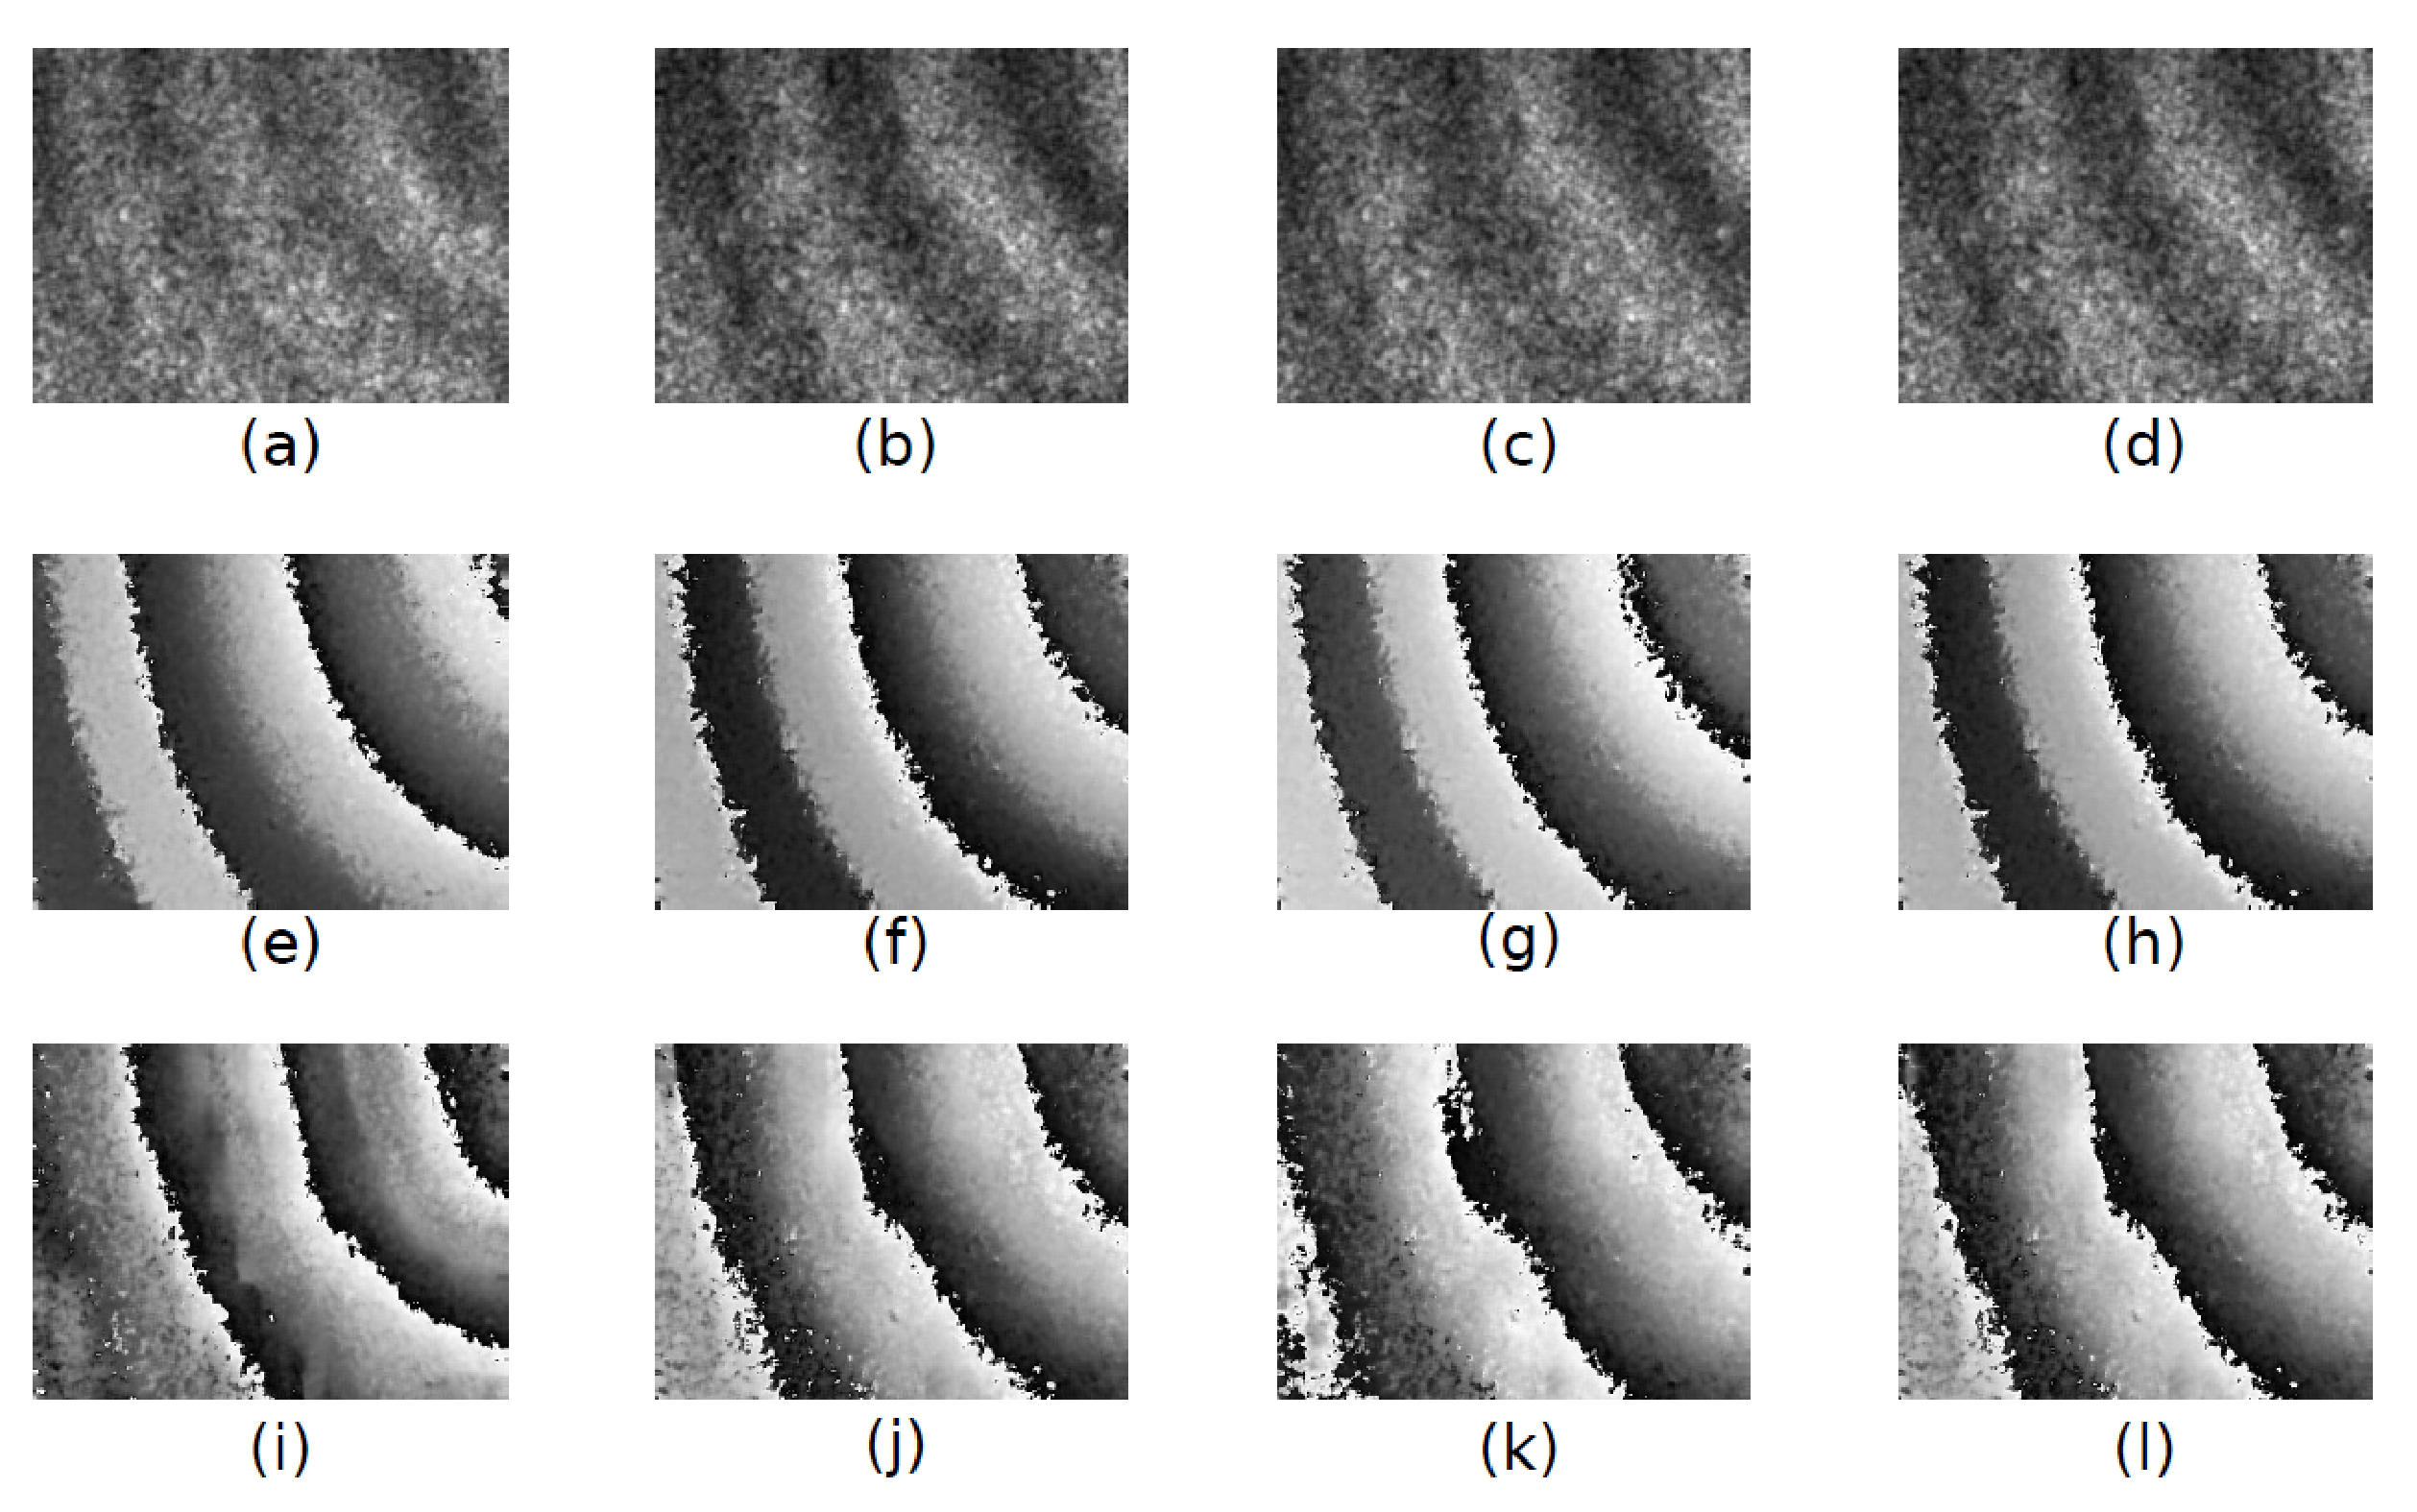
\includegraphics[scale=0.3]{Chpt3_figures/fig_3.eps}
	\end{center}
	\caption{Experimental tests.From (a) to (d) we show the interferogram
	sequence. From (e) to (h) we show the estimated wavefront using the AIA,
	and from (i) to (l) we show the estimated wavefront using the RAPS.} 
	\label{fig:ExperimentalTestRAPS}
\end{figure}

\begin{figure}[th!]
	\begin{center}
		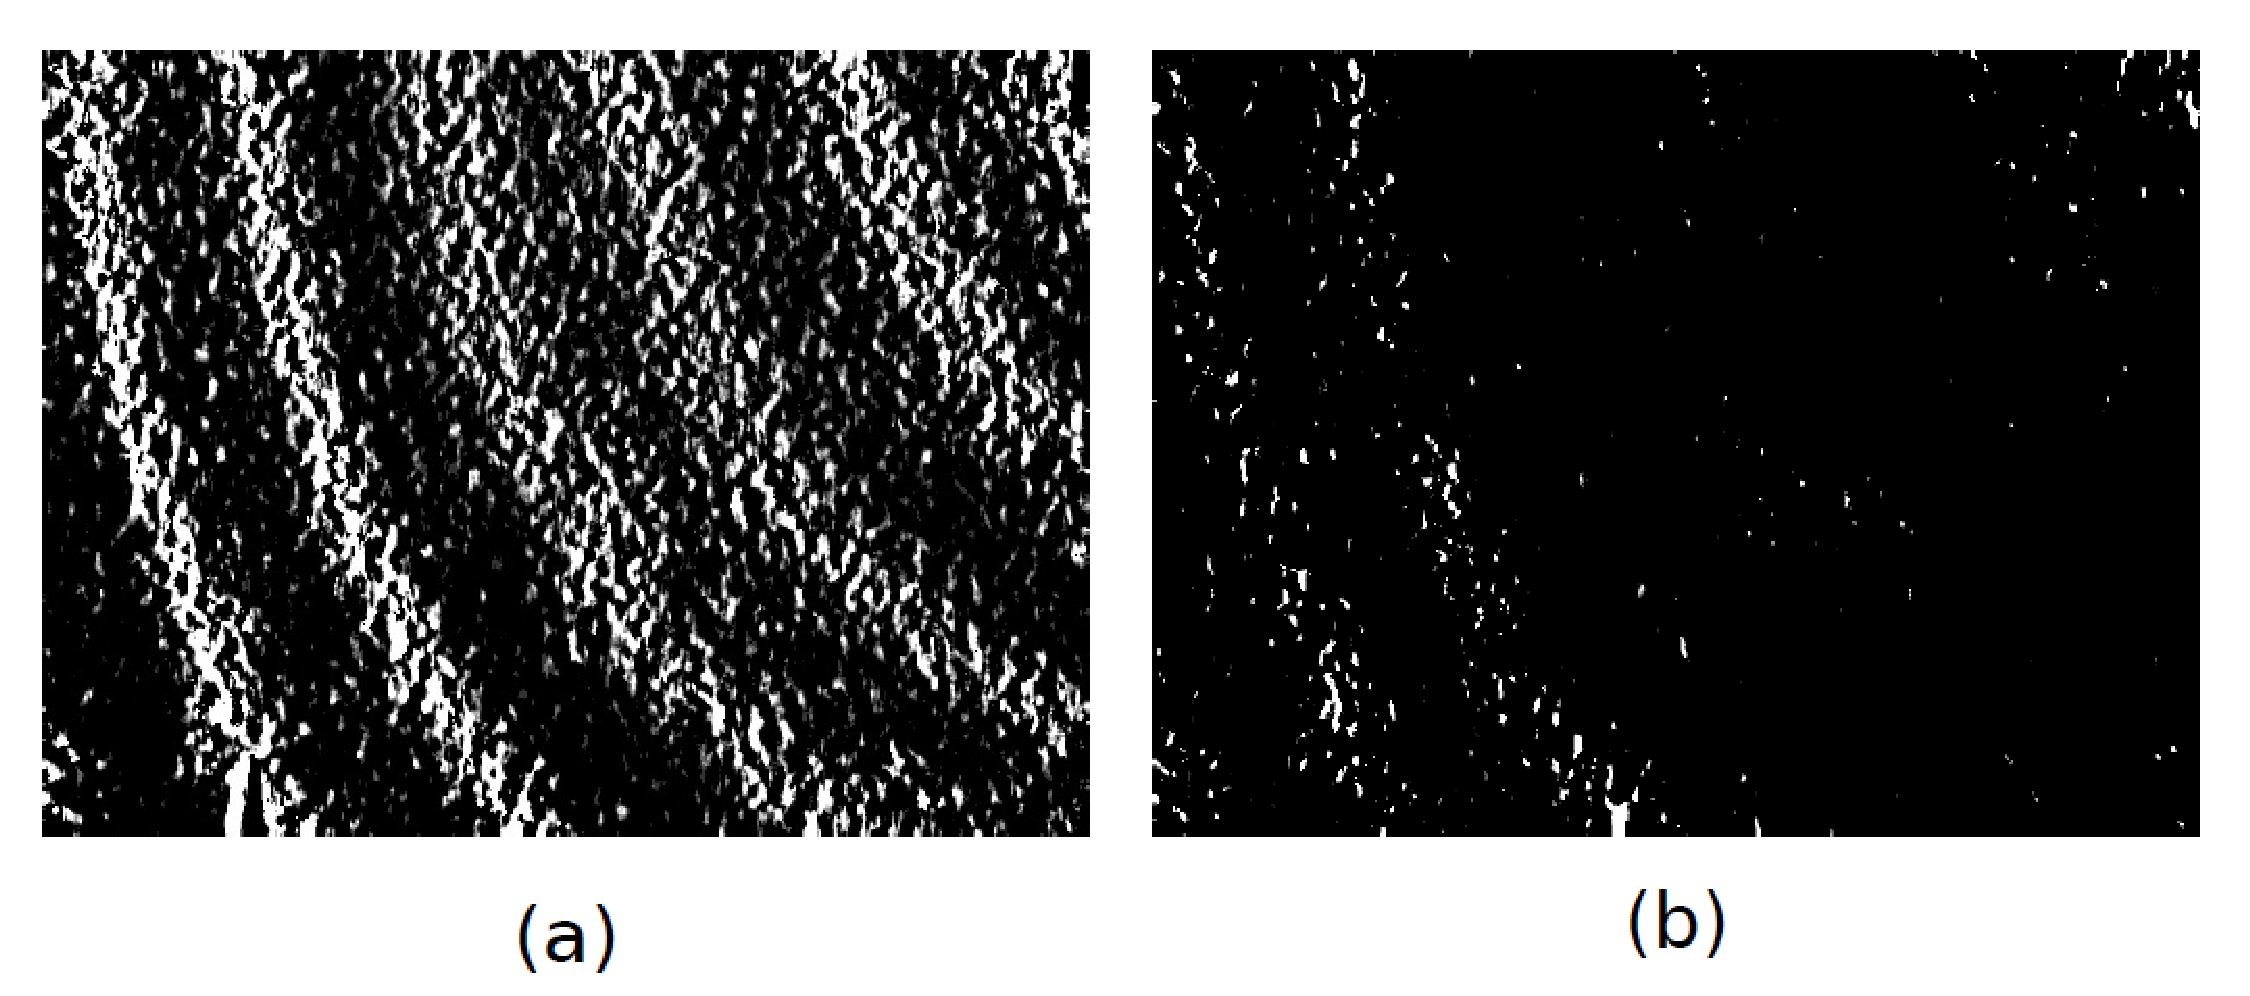
\includegraphics[scale=0.3]{Chpt3_figures/fig_4.eps}
	\end{center}
	\caption{Phase difference with respect to x (partial approximated
	derivative). The dynamic range of the difference is quantized to the
	gray levels 1, 102, 153, 203 and 255, for a better appreciation of the
	detuning error. (a) shows the phase difference corresponding to the AIA
	and (b) shows the difference corresponding to RAPS method.}
	\label{fig:DynamicRAPS}
\end{figure}

\section{Discussion and commentaries}

Accuracy of the wavefront estimation is the most important issue in optical
tests. When using PSI techniques, the estimation
accuracy depends on the stability of the object under test and the right
calibration of the PSI setup. When the wavefront under test is moving, being by
the environment perturbations or by its own nature, phase-shifting algorithms
introduce an unavoidable detuning error. Previous to this work, all
phase-shifting algorithms make the phase estimation by assuming an static
wavefront and a global phase shifting. For example, the following very known
four-steps phase-shifting algorithm:
\begin{equation}
 \phi = \arctan \Bigg( \frac{I_0-I_2}{I_1-I_3} \Bigg).
\end{equation}
This formula is the same for all pixels $(x,y)$ because it is assumed that all
pixels has the same phase shift of $\pi/2$ radians, and the modulating phase is
spatially static. However, this is not true when the wavefront under test is
moving, in this case, each pixel should have its own phase-shifting
formula/algorithm. When the wavefront under test is moving, even a self-tuning
or self-calibrating method like the one presented in
Refs.\cite{Xu:06,Wang:04,Estrada:10} introduce detuning errors. As
shown in the results, the demodulation method presented here
reduces considerably detuning errors by estimating the modulating phase and its
non constant variations for each interferogram. These estimations are made by
using iteratively the linear systems of Eqs. (4.6) and (4.9). The linear system
of Eq. (4.6) looks very similar to the one used in Ref. \cite{Wang:04}
firstly proposed in Ref. \cite{Morgan}, but, there is a big difference in the
propose of this paper. The main difference is that the phase-shifting of Eq.
(4.6) depends on the pixel $(x,y)$ being processed and
is not constant as supposed in \cite{Wang:04}. Nevertheless, the most
important contribution of the Robust Adaptive Phase-Shifting (RAPS) method
presented here, is with the Eqs. (4.7) and (4.9). The Eq. (4.7) is a weighted
least-squares cost function expressed as a quadratic convolution with a kernel
that weights the local neighborhood that will be used for the phase-shifting
estimation at the pixel $(x,y)$ of the k-interferogram. In this way, we estimate
the phase-shifting at each pixel of the k-interferogram and not a global
phase-shifting as in Refs. \cite{Xu:06,Wang:04}.

The kernel $h$ in Eq. (4.7) defines the local weighted neighborhood that is
taken into account by the least-squares function for each pixel $(x,y)$. For
example, suppose that you use a kernel with ones with the same dimension than
the interferograms. If we take the convolution of the least-squares error with
this kernel and evaluate it at the central pixel, we will have the classic
global least-squares error used in phase-shifting. Then, the size of the kernel
$h$ affects directly the results of the demodulation method presented here. As
greater it is, the results will be more comparable with the AIA method for
example and it will be less tolerant with the movements of the wavefront under
test. The convergence error of the RAPS does not depends on the h kernel
size, but the results of the demodulated phase does. If the kernel size is too
small, we do not obtain the demodulated phase as expected.

On the other hand, when the wavefront is actually not temporal static but
dynamic, its model in a local neighborhood around a time $t_0$ is the following:
\begin{equation}
 \phi(x,y,t)= \phi(x,y,t_0) + \frac{\partial \phi(x,y,t_0) }{\partial t}
 (t-t_0).
\end{equation}

In this case, the perturbation $\eta_k(x,y)$ shown in Eq. (4.2) corresponds to
the local temporal variation of the wavefront in that interferogram, that is,
$\eta_k (x,y)= \frac{\partial \phi(x,y,k\Delta t)}{\partial t} k \Delta t$,
being $\Delta t$ the discretization of the temporal $t$ variable. As a
consequence, this method can be used for testing dynamic events, regarding that
the phase shifting introduced is greater than the maximum $\eta_k(x,y),\forall
k$. Actually, the simulated wavefront given in Eq. (4.11) is a dynamic
two-modes vibrating plate. We generated the interferograms with that wavefront
model and introduced a phase-shifting of $\pi/2$ radians. As the reader can
see in the first test, we have reduced considerably the estimations errors when
the wavefront under test is moving.

Summing up, here we have presented a Robust Adaptive Phase-Shifting (RAPS)
algorithm that estimates the wavefront under test regardless its movements by
environment perturbations. However, this method can be used for testing dynamic
events using PSI techniques and with an appropriate phase-shifting. This method
estimates the wavefront under test and its non-constant variations given in each
interferogram. Compared with a traditional self-tuning phase-shifting algorithm,
this method makes better estimations by reducing considerably the detuning
errors when the wavefront under test is moving.
